%----------------------------------------------------------------------------
\chapter{Tesztelési terv}
%----------------------------------------------------------------------------

%----------------------------------------------------------------------------
\section{Időzített automata generátor tesztelése}
%----------------------------------------------------------------------------

A generált időzített automaták forráskódját unit tesztek segítségével szeretnénk tesztelni.
Az Xtext keretrendszer által nyújtott eszközök erre célra jól alkalmazhatók.

\begin{figure}[!ht]
    \centering
    
\includegraphics[width=150mm, height=9cm, keepaspectratio]{figures/unit_test_flow.png}
    \caption{Unit tesztelés folyamatábrája.}
\end{figure}

A 9.1. ábrán látható a unit tesztelés tervének folyamatábrája.
A teszteléssel az a célunk, hogy minél nagyobb magabiztosággal biztosítjuk a generátor helyes működését.
Tesztelési kategoriák:

\begin{itemize}
    \item Üzenet típusok egyenkénti tesztelése
    \item Üzenet típusokból összeállított kombinációk tesztelése
    \item Scenario operátorok tesztelése
\end{itemize}

Az üzenet típusok egyenkénti tesztelésénél az összes üzenet típust le szeretnénk fedni.
Az üzenet kombinációkból a főbb eseteket szeretnénk tesztelni.
Például a 3 üzenet típus lehetséges sorrendjeinek kombinációi.
A scenario operátoroknál azt fontos tesztelni, hogy a különálló üzenetekhez tartozó automata minták jól illeszkedjenek az operátorral elátott üzenetek automatájával.
Például sima üzenet után következik egy alt konstrukció vagy esetleg egy loop után egy elvárt üzenet.

Egy unit teszt akkor sikeres ha a generált automata forráskódja megegyezik az elvárt automata forráskódjával.
Az elvárt automata forráskódját egy korábbi generálásból adjuk meg.
Manuálisan győződünk meg a forráskód helyeségéről.

%----------------------------------------------------------------------------
\clearpage\section{Monitor forráskód generátor tesztelése }
%----------------------------------------------------------------------------

A generált monitor forráskodját integrációs tesztek segítségével szeretnénk tesztelni.
A teszteinkben egy példa rendszer java implementációját integráljuk a generált monitor komponenssel.
Az Xtext keretrendszer a specifikált DSL (Domain Specific Language) nyelvhez generál egy Maven plugin-t.
Ezt a plugin-t betölthetjük egy egyszerű maven projektbe és használhatjuk is az elkészített DSL nyelvünket, azaz létrehozhatunk a projektben a saját DSL-ünkhöz tartozó fájlokat, melyekben megadhatjuk saját scenario-inkat.

\begin{figure}[!ht]
    \centering
    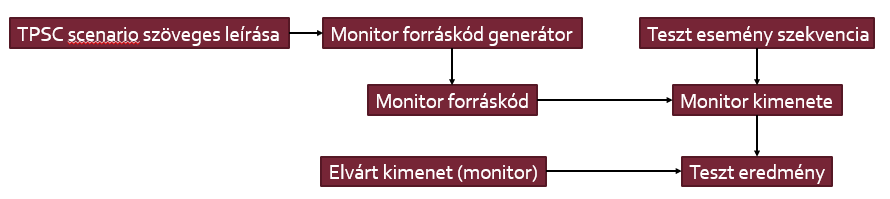
\includegraphics[width=150mm, height=9cm, keepaspectratio]{figures/integration_test_flow.png}
    \caption{Integrációs tesztelés folyamatábrája.}
\end{figure}

A 9.2. ábrán megtekinthető az integrációs tesztelés tervének folyamatábrája.
A következők tesztelési kategoriáink:

\begin{itemize}
    \item Scenario operátorok tesztelése
    \item Üzenet paraméterek tesztelése
    \item Időzítések tesztelése
\end{itemize}

A scenario operátorok tesztelésénél az a célunk, hogy a monitor a követelmény különböző ágait figyelembe véve helyes kimenetet adjon.
Például loop operátor esetén a minimum, köztes és maximum üzenet szekvencia ismétléseknél is helyes legyen a monitor kimenete.
Ha a maximumnál többször szerepel az üzenet szekvencia akkor hibát kell, hogy jelezen.
Üzenet paraméterek tesztelése esetén azt szeretnénk vizsgálni, hogy a monitor helyesen értelmezi e az üzenet paramétereket.
Az időzítések tesztelésénél az a fontos, hogy a monitor képes-e az óraváltozók alapján az időzitési feltételeket kiértékelni.
Például ha az üzenet a feltétel alapján időben érkezik meg akkor helyes kimenetet adjon vissza ha feltétel szerint később érkezik meg akkor a monitornak hibát kell jeleznie.

Egy integrációs teszt akkor sikeres ha a monitor kimenete megegyezik az elvárt kimenettel.
Az elvárt kimenetet a rendszer manuális tesztelése határoz meg.
A tesztelő dönti el, hogy helyesen kell hogy működjön vagy sem amit a monitornak jeleznie kell.

%----------------------------------------------------------------------------
\clearpage
%----------------------------------------------------------------------------

Az Xtext keretrendszer a definiált DSL nyelvünkhöz generál egy Maven projekt architektúrát.
A nyelvünk így elérhető maven plugin formájában is, amit felhasználhatunk az integrációs teszteinkhez.
Elég csupán egy maven projektet felkonfigurálni a saját dsl plugin-ünkkel és elkészítethetjük a saját tesztelési keretrendszerünket.
A 9.3. ábrán és a 9.1. kódrészléten látható egy ilyen integrációs teszthez tartozó maven projekt felépítése és a hozzá tartozó teszteset.

\begin{figure}[!ht]
    \centering
    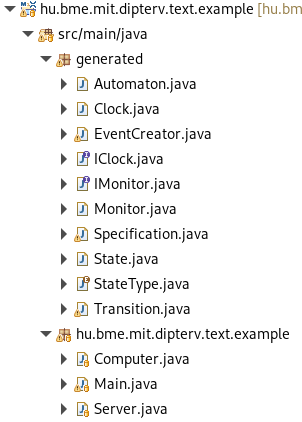
\includegraphics[width=150mm, height=9cm, keepaspectratio]{figures/integration_test_structure.png}
    \caption{Példa integrációs teszt projekt struktúrája.}
\end{figure}

\begin{lstlisting}[language=java, frame=single, float=ht!, caption={Integrációs teszteset.},captionpos=b]
package hu.bme.mit.dipterv.text.example;

import org.junit.jupiter.api.Test;
import org.junit.jupiter.api.Assertions;

import generated.Specification;
import generated.IClock;
import generated.IMonitor;
import generated.Monitor;
import generated.Clock;

public class MonitorPassingTest {

	@Test
	public void testMonitorPassing() {
		Specification specification = new Specification();
		specification.listAutomatas();
		IClock clock = new Clock();
		IMonitor monitor = new Monitor(specification.getAutomata().get(0), clock);

		Server server = new Server(monitor);
		Computer computer = new Computer(server, monitor);
		Assertions.assertTrue(monitor.goodStateReached());
	}
}
\end{lstlisting}

\begin{lstlisting}[language=java, frame=single, float=ht!, caption={Integrációs teszteset eredménye.},captionpos=b]
-------------------------------------------------------
T E S T S
-------------------------------------------------------
Running hu.bme.mit.dipterv.text.example.MonitorPassingTest
q0 NORMAL
q1 NORMAL
q2 ACCEPT
q3 NORMAL
q4 NORMAL
q5 FINAL
!(computer.checkEmail().computer) q0->q0
computer.checkEmail().computer q0->q1
!(computer.sendUnsentEmail().server) q1->q1
!(computer.sendUnsentEmail().server) q1->q2
computer.sendUnsentEmail().server q1->q3
!(computer.logout().server) & !(computer.newEmail().server) q3->q3
computer.newEmail().server q3->q4
!(computer.downloadEmail().server) q4->q4
computer.downloadEmail().server q4->q5
Received Message: computer.checkEmail().computer
Transition: !(computer.checkEmail().computer)
Transition: computer.checkEmail().computer
transition triggered: computer.checkEmail().computer
q1

Received Message: computer.sendUnsentEmail().server
Transition: !(computer.sendUnsentEmail().server)
Transition: !(computer.sendUnsentEmail().server)
Transition: computer.sendUnsentEmail().server
transition triggered: computer.sendUnsentEmail().server
q3

Received Message: computer.newEmail().server
Transition: !(computer.logout().server) & !(computer.newEmail().server)
Transition: computer.newEmail().server
transition triggered: computer.newEmail().server
q4

Received Message: computer.downloadEmail().server
Transition: !(computer.downloadEmail().server)
Transition: computer.downloadEmail().server
transition triggered: computer.downloadEmail().server
q5

Tests run: 1, Failures: 0, Errors: 0, Skipped: 0, Time elapsed: 0.025 sec

Results :

Tests run: 1, Failures: 0, Errors: 0, Skipped: 0
\end{lstlisting}

A 9.2. kódrészlet a Maven teszt kimenetét tartalmazza.

Ezt a projekt struktúrát felhasználva a teszteink köré tudunk egy Maven alapú Continuous Integration (CI) állítani.

A függelékben található egy példa unit teszt eset az automata generátor tesztelésére.